% -----------------------------------------------------------------------------------------|
\documentclass[a4paper,11pt,titlepage,twoside,openany]{book}

% draft: comando che mostra i problemi di sillabazione e giustificazione con un quadratino nero, inoltre non carica le immagini, così compila più velocemente VA TOLTO PRIMA DI CONSEGNARE O PER VISUALIZZARE LE IMMAGINI

%
\usepackage{plain}
\usepackage{setspace}
\usepackage{geometry} % per definizione layout
\usepackage{titlesec} % per formato custom dei titoli dei capitoli
\usepackage[utf8x]{inputenc}
\usepackage{graphicx} % Gestione immagini
\usepackage{wrapfig} % Immagini con testo a lato
\usepackage{booktabs} % Migliore gestione delle tabelle
\usepackage{caption}% Migliore gestione delle didascalie
\usepackage{float} % Forzatura posizione tabelle
\usepackage[english]{babel}
\usepackage{lipsum}  
\usepackage{afterpage}
\usepackage{comment}
\usepackage{eurosym}
\usepackage[export]{adjustbox}
\usepackage{url}
\usepackage{etoolbox}
\usepackage{afterpage}
\usepackage{graphicx}
\usepackage{titling}
\usepackage{datetime}
\usepackage{subcaption}
\usepackage{amsmath}
\usepackage{amsfonts}
\usepackage{wrapfig}
\usepackage{hyperref}
\usepackage{array}
\usepackage{geometry}
\usepackage{listings}
\usepackage{xcolor}
\usepackage{svg}


\newcommand\blankpage{%
    \null
    \thispagestyle{empty}%
    \addtocounter{page}{-1}%
    \newpage} % importo pacchetti
\singlespacing
%
\begin{document}
%%%
%
%-----------------------|
%                       |
%       TITLE PAGE      |
%                       |
%-----------------------|
%
%%%
  \newgeometry{outer=2cm,inner=2cm,top=2cm,bottom=2cm, hmarginratio=1:1} 
  \pagenumbering{gobble} 
  \pagestyle{plain}
\thispagestyle{empty}

  \vspace*{\fill}

  \begin{center}
  \begin{figure}[h!]
    %\centerline{
\psfig{file=marchio_unitrento_colore_it_202002.eps,width=0.6\textwidth}}
    \centering
    
\includegraphics[keepaspectratio, width=0.6\textwidth]{Pic/marchio_unitrento_colore_it_202002.eps}
  \end{figure}

  \vspace{2 cm} 

  \LARGE{Advanced Programming of Cryptographic Methods}\\

  \vspace{1 cm} 
  \Large{Project Report}

  \vspace{2 cm} 

  \Huge\textsc{IdenCA\\ An Identity Certificate Authority}

    \vspace{2 cm} 

  \Large{\it{ Emanuele Civini, Alessia Pivotto }}

  \vspace{2 cm} 

  \Large{Academic year 2024/2025}
  \vspace*{\fill}
\end{center}

  \clearpage
%  
%%%
%%%%%%%%%%%%%%%%%%%%%%%%%%%%%%%%%%%%%%%%%%%%%%%%%%%%%%%%%%%%%%%%%%%%%%%%%%
%%%
%
%------------------------|
%                        |
%         INDICE         |
%                        |
%------------------------|
%
%%%
    \mainmatter
    \newgeometry{outer=2cm,inner=2.6cm,top=2.5cm,bottom=2.5cm, foot = 1.2cm}
    \tableofcontents
    \clearpage 
    \newpage
%----------------------------------------------------------------------------------|
%%%%%%%%%%%%%%%%%%%%%%%%%%%%%%%%%%%%%%%%%%%%%%%%%%%%%%%%%%%%%%%%
    % gruppo per definizone di successione capitoli senza interruzione di pagina
    \begingroup
      % nessuna interruzione di pagina tra capitoli
      
     \makeatletter
     \patchcmd{\chapter}{\if@openright\cleardoublepage\else\clearpage\fi}{\par}{}{}
     \makeatother
      
      % redefinizione del formato del titolo del capitolo
      % da formato
      %   Capitolo X
      %   Titolo capitolo
      % a formato
      %   X   Titolo capitolo

      \titleformat{\chapter}{\normalfont\Huge\bfseries}{\thechapter}{0.6cm}{}
        
      \titlespacing*{\chapter}{0pt}{0.5in}{0.2in} % originale {0pt}{0.59in}{0.02in}
      \titlespacing*{\section}{0pt}{0.3in}{0.10in} % originale {0pt}{0.20in}{0.02in}
      \titlespacing*{\subsection}{0pt}{0.10in}{0.05in} % originale {0pt}{0.10in}{0.02in}
%%%%%%%%%%%%%%%%%%%%%%%%%%%%%%%%%%%%%%%%%%%%%%%%%%%%%%%%%%%%%%%%
%%%
%
%----------------------|
%                      |
%       SOMMARIO       |
%                      |
%----------------------|
%
%%%
    \chapter{Introduction}
\label{ch:introduction}
This project implements a Certificate Authority (CA) system that manages digital certificates for 
secure communications. A CA is a trusted entity that issues digital certificates to verify the identity 
of users and the possession of a private key.
The system provides a complete solution for certificate management, including issuing new certificates, 
checking their validity, renewing them before expiration, and revoking them when necessary. 
The implementation focuses on security by using an Hardware Security Module (HSMs) to protect
the CA's private key and implementing proper verification procedures.
The system provides user-friendly interfaces through both API endpoints for developers and a web 
interface for end users. 

\section{Key Features}

The Certificate Authority supports the complete certificate lifecycle. 
For certificate issuance, the system processes certificate requests, verifies the requester's identity, 
and issues signed certificates. 
It provides certificate validation by checking if certificates are valid, not expired, and haven't been revoked.

The system allows users to renew their certificates before they expire and handles certificate revocation 
for compromised or no longer needed certificates, maintaining a Certificate Revocation List (CRL). 
Identity verification ensures that certificate requesters own the private key and control the email 
address associated with their request.

\section{System Architecture}

The system consists of several integrated components. The backend server is a Go API that handles 
all certificate operations and communicates with the database and HSM. 
A Next.js frontend application provides an easy-to-use web interface for certificate management.

Data persistence is handled by MongoDB storage for certificate records, user commitments, and system data. 
Security operations are performed by a HSM that stores the CA's private key 
and performs cryptographic operations. 
An automated email service supports identity verification during certificate requests.

\section{Report Structure}

This report provides a comprehensive overview of the Certificate Authority implementation. 
Chapter 2 presents the requirements analysis and system specifications. 
Chapter 3 details the system design and architecture. 
Chapter 4 covers implementation details and technology choices, while Chapter 5 discusses security 
considerations and best practices. 
Finally, Chapter 6 provides deployment guidance and usage instructions.

Each chapter builds upon the previous one, providing a complete understanding of the Certificate 
Authority from idea to deployment.
% citazione sennò latex si spacca tutto 
    \newpage
    \chapter{Requirements}

This chapter defines the requirements for our Certificate Authority, 
categorized into functional and security requirements. Each requirement focuses 
on what the system must accomplish rather than implementation details.

\section{Functional requirements}

The functional requirements define the core capabilities that the Certificate 
Authority must provide to fulfill its role.

\subsection{FR1: Certificate issuance}

The CA must generate and issue digital certificates after verifying the 
identity of the certificate requester. This includes:

\begin{itemize}
    \item Receiving and validating certificate requests
    \item Verifying the authenticity of certificate requests
    \item Generating X.509 compliant certificates
\end{itemize}

Certificate issuance is the foundation of a certificate authority, 
requiring identity verification to prevent unauthorized issuance.

\subsection{FR2: Certificate revocation}

Users must be able to request revocation of their certificates at any time, 
particularly when suspecting private key compromise. The system shall:

\begin{itemize}
    \item Accept authenticated revocation requests from certificate holders
    \item Verify proof of private key ownership before processing revocation
    \item Immediately update the certificate status upon successful verification
\end{itemize}

This capability ensures certificate holders maintain control over their 
digital identities and can respond quickly to security incidents.

\subsection{FR3: Certificate Revocation List (CRL) accessibility}

The CA must maintain and publish a Certificate Revocation List that allows 
anyone to verify certificate status. Requirements include:

\begin{itemize}
    \item Maintaining an up-to-date list of all revoked certificates
    \item Providing public access to CRL information
    \item Digitally signing the CRL to ensure authenticity
\end{itemize}

Public CRL access enables relying parties to perform proper certificate validation.

\subsection{FR4: Identity verification}

The CA must verify both email authenticity and private key ownership for 
certificate applicants. This simplified verification process includes:

\begin{itemize}
    \item Email verification through challenge-response mechanisms
    \item Private key ownership verification via cryptographic challenges
\end{itemize}

This approach provides reasonable assurance that certificate requests come 
from legitimate key-holders controlling the specified email addresses.

\subsection{FR5: Public key publishing}

The CA must publish issued certificates and its own public key to enable 
certificate validation. This requires:

\begin{itemize}
    \item Maintaining a publicly accessible certificate repository
    \item Publishing the CA's public key as a trust anchor
    \item Providing standard interfaces for certificate retrieval
\end{itemize}

Public availability of certificates and the CA public key enables the complete 
certificate validation process for all relying parties.

\subsection{FR6: Certificate renewal}

The CA must support certificate renewal before expiration to ensure service 
continuity. The renewal process shall:

\begin{itemize}
    \item Verify the current certificate has not been revoked
    \item Perform identity verification equivalent to initial issuance
    \item Ensure proper timing to prevent service interruptions
\end{itemize}

Renewal maintains trust relationships beyond individual certificate lifespans 
while preserving security through re-verification.

\subsection{FR7: Cryptographic algorithm support}

The CA must support both RSA and ECDSA cryptographic algorithms to ensure 
broad compatibility:

\begin{itemize}
    \item RSA support with minimum 2048-bit key sizes
    \item ECDSA support using the P-256 curve
    \item Key generation, signing, and verification for both algorithms
\end{itemize}

Multi-algorithm support accommodates diverse client requirements and provides 
flexibility for different security and performance needs.

\section{Security requirements}

Security requirements define the protective measures the Certificate Authority 
must maintain to ensure service integrity, confidentiality, and 
availability.

\subsection{SR1: Certificate authenticity}

Certificates containing valid CA signatures must be considered authentic and 
trustworthy. This requires:

\begin{itemize}
    \item Cryptographically strong signature algorithms
    \item Secure certificate signing procedures
    \item Readily available signature verification mechanisms
\end{itemize}

Certificate authenticity forms the foundation of PKI trust, enabling relying 
parties to confidently validate certificate legitimacy.

\subsection{SR2: Certificate validity verification}

Expired certificates and those appearing in the CRL must be considered invalid 
regardless of signature authenticity. Validation must include:

\begin{itemize}
    \item Expiration date verification for temporal validity
    \item CRL consultation for revocation status
    \item Clear rejection of certificates failing either test
\end{itemize}

Comprehensive validity checking prevents acceptance of certificates that may 
pose security risks despite technical authenticity.

\subsection{SR3: Secure key management}

The CA private key must be protected using Hardware Security Modules (HSMs) 
with the following protections:

\begin{itemize}
    \item Tamper-resistant hardware storage
    \item Protection against unauthorized access and extraction
    \item All signing operations performed within the HSM boundary
    \item Comprehensive audit trails of key usage
\end{itemize}

HSM protection ensures the CA private key, the most critical PKI asset, 
remains secure against various attack vectors.

\subsection{SR4: Data integrity and confidentiality}

All certificate data, configuration, and audit logs must be protected against 
unauthorized access and modification:

\begin{itemize}
    \item Database encryption for stored information
    \item Secure communication protocols for data transmission
    \item Access controls and integrity checking mechanisms
\end{itemize}

Data protection ensures certificate information remains accurate and prevents 
inappropriate disclosure of sensitive information.

These requirements collectively define the functional capabilities and security 
posture necessary for effective and secure Certificate Authority operations.    
    \newpage
    \chapter{System architecture and certificate lifecycle}
\label{Architecture}

This chapter presents the architectural design decisions and  operational flows 
of the Certificate Authority. The focus is on explaining how the various 
components interact throughout the complete certificate lifecycle, from initial 
identity commitment to certificate issuance, renewal, and revocation.


\section{Source code structure}

The system consists of four primary components, each serving a specific role in 
the certificate lifecycle:

\subsection{CA backend server} 
The core service responsible for all cryptographic operations and certificate 
lifecycle management. Go was selected for its strong and complete cryptographic standard library, 
excellent performance characteristics and simplicity of development.

\subsection{User interface}
A React-based frontend providing certificate management capabilities. As this UI is intended 
to be used only for demo purposes, Next.js was chosen for its ease of use, built-in routing 
and vast ecosystem of libraries.

\subsection{Database}
Persistent storage for certificates and revocation lists. We decided to use MongoDB for its
document-oriented structure, which allows flexible storage and suits well with the certificate and 
metadata requirements. It also provides indexing capabilities for efficient 
querying and retrieval of certificate data.

\subsection{Hardware Security Module (HSM)}
We decided to use an HSM, in particular an emulated version of AWS KMS, to ensure that all CA 
cryptographic operations requiring its private key occur within FIPS 140-2 Level 3 certified hardware. 
This design decision eliminates the risk of private key exposure while providing 
enterprise-grade security and audit capabilities.

\section{Security-first architecture}
The architecture implements security principles through multiple 
layers of protection.

\subsection{Cryptographic isolation}
The CA's root private key never exists outside 
the HSM boundary. All signing operations are performed through secure API calls 
to the HSM, ensuring the key material remains protected even if other system 
components are compromised.

\subsection{Identity verification}
A two-step identity verification process combines 
email ownership verification with cryptographic proof of private key possession. 
This dual verification ensures only legitimate key owners can obtain certificates.

\subsection{Signed responses}
Critical CA responses are cryptographically signed to ensure 
integrity and authenticity. This prevents response tampering and provides 
non-repudiation for all CA operations.

\subsection{Replay protection}
Nonce-based replay protection mechanisms prevent 
malicious reuse of previously captured requests, protecting against replay attacks.

\section{Certificate lifecycle operations}

This section details the complete certificate lifecycle, explaining the message 
flows, cryptographic operations, and component interactions for each phase.

\subsection{Phase 1: identity commitment}

The certificate issuance process begins with an identity commitment phase that 
establishes and verifies user identity through a multi-step protocol.

\subsubsection{Client-side operations}

The user commits their identity by sending their public key, PEM-encoded,
along with their email address.

\subsubsection{CA backend processing}

When the CA backend receives the commitment request at the `/v1/identity` 
endpoint, it performs comprehensive validation.
The system validates the email address format using standard RFC 5322 compliance 
checking. The public key undergoes cryptographic validation 
to ensure it is valid and properly formatted.

Upon successful validation, the CA generates a unique challenge string and creates 
an identity commitment record in the database. This record contains the user's 
email, public key in DER format, challenge string and an 
expiration timestamp. The CA reserves a unique serial number for the eventual 
certificate, ensuring no conflicts occur during concurrent requests. An identity
commitment is valid for the next 24 hours, after which it expires and must be 
re-committed. In addition, it's not possible to verify the same identity twice.

\subsubsection{Email verification}

The identity verification process leverages email ownership as proof of identity. 
The CA's email service sends the challenge string, encoded in base 64, to the user's provided email 
address using a secure email delivery service.
This email-based verification serves dual purposes: it confirms the user has 
access to the claimed email address and provides the challenge string needed 
for the subsequent cryptographic proof phase.

\subsection{Phase 2: certificate generation}

The certificate generation phase requires cryptographic proof of private key 
ownership before the CA will issue a certificate.

\subsubsection{Challenge response}

After receiving the challenge via email, the user returns to the certificate 
interface and provides the challenge string. The client application retrieves 
the challenge and prompts the user to sign it using their private key.
The signing operation occurs entirely within the browser using the Web Crypto API. 
The client signs the raw challenge bytes using the private key corresponding to 
the public key submitted during commitment. This creates a digital signature 
that proves the user possesses the private key without exposing it.

\subsubsection{CA verification and certificate issuance}

The CA receives the challenge response containing the challenge string and the 
cryptographic signature. The system performs several critical verification steps.
First, the CA retrieves the identity commitment record using the provided challenge. 
It verifies the commitment hasn't expired and hasn't been previously used, 
preventing replay attacks and ensuring temporal validity.
Next, the CA performs signature verification using the public key from the 
commitment record. This cryptographic verification proves the requester possesses 
the corresponding private key. The verification process uses the appropriate 
algorithm (ECDSA or RSA) based on the committed key type.

Upon successful verification, the CA initiates certificate generation. The system 
constructs an X.509 certificate containing the user's public key, email address 
as the subject, and the reserved serial number. The certificate includes standard 
extensions such as key usage, basic constraints, and subject alternative names.

\subsubsection{HSM-Based certificate signing}

The certificate signing operation represents the most security-critical component 
of the entire system. The CA never signs certificates using local private keys; 
instead, all signing operations occur within the Hardware Security Module.
The CA formats the certificate structure and sends it to the HSM through the 
AWS KMS API. The HSM performs the cryptographic signing operation using the 
CA's root private key, which never leaves the secure hardware boundary. This 
approach ensures the highest level of security for the CA's signing operations.
The HSM returns the signature, which the CA combines with the certificate data 
to produce the final signed X.509 certificate. The completed certificate is 
returned to the client in PEM format, ready for immediate use.

\subsection{Phase 3: certificate revocation}

Certificate revocation enables certificate owners to invalidate their certificates 
before their natural expiration, essential for handling key compromise or 
changing security requirements.

\subsubsection{Revocation request authentication}

The revocation process begins when a certificate owner accesses the revocation 
interface and provides their certificate's serial number. The system requires 
cryptographic proof that the requester owns the certificate's corresponding 
private key.
The client constructs a revocation message in the format "Revoke: $<$serial number$>$" 
where the serial number matches the certificate being revoked. The user signs 
this message using their private key, creating a revocation signature that 
proves their authority to revoke the certificate. A nonce is not required in this
case because the operation can be performed only once per certificate.

\subsubsection{CA revocation processing}

The CA receives the revocation request containing the serial number and signature. 
The system retrieves the original identity commitment record associated with 
the serial number to obtain the corresponding public key.
The CA verifies the revocation signature against the constructed message 
"Revoke: $<$serial number$>$" using the certificate's public key. This verification 
ensures only the legitimate certificate owner can initiate revocation.

Upon successful verification, the CA updates the certificate record in the database, 
marking it as revoked with the current timestamp. The revoked certificate is 
immediately added to the Certificate Revocation List (CRL), making the revocation 
status publicly available through the CRL endpoint.

\subsection{Phase 4: certificate renewal}

Certificate renewal allows users to extend their certificate validity period 
without generating new key pairs, maintaining continuity while refreshing 
the certificate's temporal validity.

\subsubsection{Renewal request process}
The renewal process requires the certificate owner to prove continued possession 
of the private key. The client constructs a renewal message in the format 
"Renew: $<$serial number$>$ Nonce: $<$random nonce$>$" and signs it using the certificate's 
private key.
This signature proves the requester still controls the private key associated 
with the certificate, ensuring only legitimate certificate owners can renew 
their certificates. To avoid replay attacks, the renewal message includes a 
random nonce that must be unique for each renewal request. Subsequent requests 
for the same certificate using the same nonce will be rejected by the CA.

\subsubsection{CA renewal validation and processing}

The CA performs several validation steps before processing renewal requests.
First, the system verifies the certificate exists and hasn't been revoked. It confirms 
the certificate hasn't expired, as expired certificates cannot be renewed. 
The, the CA validates the renewal signature against the message "Renew: $<$serial number$>$ Nonce: 
$<$provided nonce$>$" using the committed public key.
Upon successful validation, the CA extends the certificate's validity period 
(typically by one year) and generates a new certificate with the updated expiration 
date. It also keeps track of the used nonces for this certificate to prevent 
replay attacks.
The renewed certificate maintains the same serial number and subject 
information while reflecting the extended validity period.

\subsubsection{HSM integration in renewal}

Similar to initial certificate issuance, the renewal process involves HSM-based 
signing operations. The CA constructs the renewed certificate structure and 
submits it to the HSM for signing using the root private key.
This ensures renewed certificates maintain the same level of cryptographic 
integrity as originally issued certificates, with all signing operations 
occurring within the secure hardware boundary.

\section{Component interactions and message flows}

This section provides detailed analysis of how system components communicate during 
certificate operations, emphasizing the role of the HSM and signed responses.

\subsection{Frontend-backend communication}

The web interface communicates with the CA backend through RESTful API endpoints, 
with each operation following specific message flow patterns.
The process starts with the identity commitment flow, where the frontend sends a POST request to 
`/v1/identity` containing the user's email and public key in PEM format. The backend responds with an HTTP 200 status upon successful 
commitment creation, triggering the email verification process.
Then, once the user has received the challenge via email and wrote it into the `Sign` section
together with the associate private key, the frontend computes the required signature and submits 
a POST request to `/v1/certificate` with the challenge string and signature. 
The backend validates the signature and returns the signed certificate in PEM format.
\begin{figure}[h!]
    \centering
    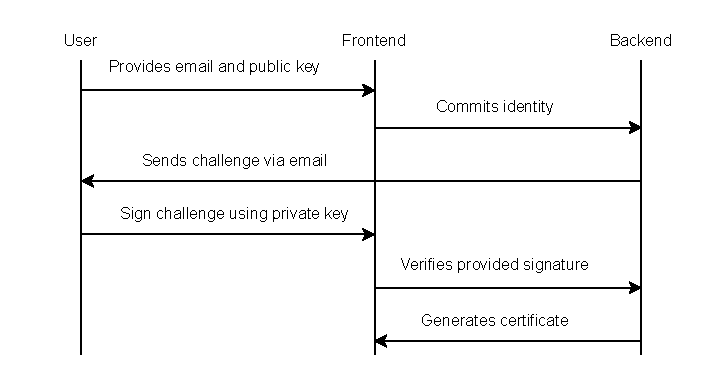
\includegraphics[keepaspectratio, width=\textwidth]{Pic/create_certificate.pdf}
    \caption{Identity commitment and certificate generation flow}
    \label{fig:certificate-creation-flow}
\end{figure}
When a user wants to revoke a certificate, the frontend sends a POST request to 
`/v1/certificate/revoke` containing the serial number of the certificate and the revocation 
signature. The backend validates the signature and confirms revocation through a JSON response.

\begin{figure}[h!]
    \centering
    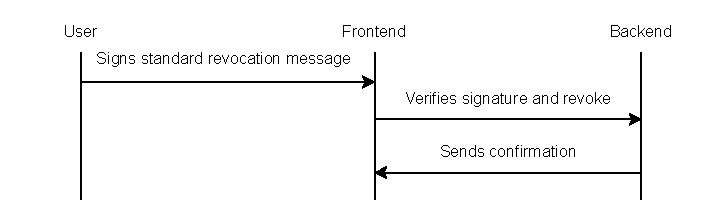
\includegraphics[keepaspectratio, width=\textwidth]{Pic/revoke_certificate.pdf}
    \caption{Certificate revocation flow}
    \label{fig:certificate-revocation-flow}
\end{figure}
Similarly, when a user wants to renew a certificate, the frontend sends a POST 
requests to `/v1/certificate/renew` containing renewal signatures and the serial number of the 
certificate. Successful renewal returns both confirmation and the renewed certificate.

\begin{figure}[h!]
    \centering
    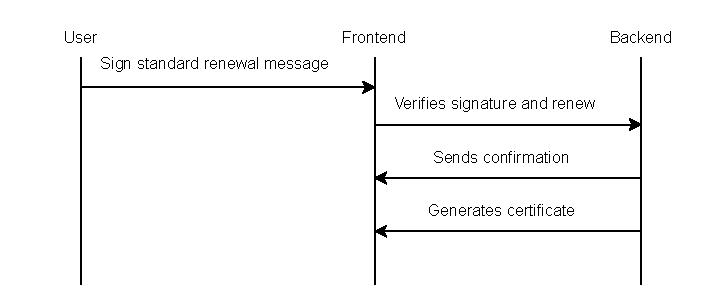
\includegraphics[keepaspectratio, width=\textwidth]{Pic/renew_certificate.pdf}
    \caption{Certificate renewal flow}
    \label{fig:certificate-renewal-flow}
\end{figure}

\subsection{HSM integration patterns}

The HSM integration follows secure communication patterns 
that ensure private key material never leaves the secure boundary:

\subsection{Key creation}
During system initialization, the CA creates a root key 
within the HSM using the AWS KMS CreateKey API. The key specification uses 
ECC NIST P-256 for its security and performance. The HSM generates the key 
pair entirely within secure hardware, returning only the key identifier.

\subsection{Certificate signing}
For each certificate signing operation, the CA 
constructs the certificate structure locally and sends it to the HSM via the 
KMS Sign API. The HSM performs the cryptographic signature using the stored 
private key and returns only the signature bytes. This pattern ensures the 
private key never exists outside the HSM boundary.

\subsection{Root certificate generation}
The system generates the CA's root certificate 
by creating the certificate structure and requesting HSM signing. The resulting 
self-signed root certificate establishes the trust anchor for all issued certificates.

\section{Signed responses}

To ensure response integrity and prevent tampering, the system implements 
OCSP-like signed responses for critical operations:

\subsection{Response structure}
Each signed response contains response data, 
signature algorithm identifier, Base64-encoded signature, and optional signing 
certificate chain. The response data includes nonces for replay protection 
and timestamps for freshness validation.

\subsection{Certificate status responses}
When clients query certificate status, 
the CA constructs a response containing the serial number, status (good/revoked/unknown), 
update timestamps, and revocation details if applicable. The complete response 
is signed using the HSM to ensure authenticity.

\subsection{Revocation list responses}
Certificate Revocation List queries return 
signed responses containing the list of revoked certificates with pagination 
support. Each response includes update timestamps and replay protection nonces.

\section{Code Structure and organization}

The project follows a monorepo structure with clear separation between different 
services and components, enabling independent development and deployment while 
maintaining code organization.

\subsection{Backend service (ca/)}
This directory contains the complete Go-based Certificate Authority 
server implementation. This module includes the REST API server, HSM integration, 
database operations, and email services. The structure follows Go's standard 
project layout with clear separation between commands, internal packages, and 
configuration. It is organized as follows:
\begin{itemize}
    \item \textbf{cmd/}: Contains the main application entry point and service 
    initialization logic.
    \item \textbf{internal/}: Core business logic modules including configuration, 
    database operations, HSM integration, email services, and HTTP server implementation.
    \item \textbf{handler/}: RESTful API endpoint implementations organized by 
    functionality (e.g., certificate operations, health monitoring).
\end{itemize}

\subsection{Frontend application (ui/)}
This directory contains the Next.js-based web interface 
providing user-facing certificate management capabilities. The structure follows 
Next.js App Router conventions with organized pages, components, and utility 
functions for cryptographic operations.
In particular:
\begin{itemize}
    \item \textbf{app/}: Contains the main application entry point, routing, and 
    layout definitions. The directory structure follows Next.js conventions with 
    pages organized by functionality.
    \item \textbf{components/}: Reusable UI components such as forms, buttons, 
    and modals used across different pages.
    \item \textbf{utils/}: Utility functions for cryptographic operations, API 
    communication, and data formatting.
\end{itemize}

\subsection{Certificates (dev-certs/)}
This directory, initially empty, contains the root certificate generated by the CA.

\subsection{Deployment configuration}
In the root directory of the project there are files including Docker Compose 
orchestration, MongoDB configuration, and environment setup scripts for 
containerized deployment.

\section{Dependencies and libraries}

The system uses external dependencies to provide robust functionality 
while minimizing security risks and maintaining code quality.

\subsection{Backend dependencies}
Go 1.21+ provides all the packages required for cryptographic operations, thanks to 
its standard library including crypto/x509, crypto/rsa, crypto/ecdsa, but also net/http 
for API server functionality.
To integrate MongoDB, we decided to use the official MongoDB Go driver (go.mongodb.org/mongo-driver/v2) 
as it provides secure and comprehensive access to MongoDB features, including 
document-oriented data storage, indexing, and querying capabilities.
For the HSM, we decided to opt for the official AWS SDK Go library (github.com/aws/aws-sdk-go-v2) 
as it provides programmatic access to AWS KMS for secure key management and signing 
operations.
Lastly, we opted for Resend Go package as it is the official client of the email delivery service
we decided to use.


\subsection{Frontend dependencies}

At the core we decided to use Next.js 15 with React 19 as it provides easy routing and
lots of UI packages with pre-built components, which allowed us to speed up the development process.
We opted for Web Crypto API (browser native) to handle 
client-side cryptographic operations without requiring external libraries.

\subsection{Infrastructure dependencies}

We opted for Docker and Docker Compose as they allow for easy and consistent deployment 
environments with isolated service containers. For the database, as we wanted a document-based one,
we decided to use MongoDB since we were already familiar with it and it provides document-oriented 
data storage with indexing, and querying capabilities for scalable management.
For the HSM, the only free solution we found was LocalStack KMS, which provides a local HSM emulation
for development and testing environments without requiring cloud resources, but emulating the AWS KMS API.

\subsection{Security and compliance dependencies}

All selected dependencies prioritize security and maintain active development 
with regular security updates. The minimal dependency approach reduces attack 
surface while leveraging proven, well-maintained libraries from reputable sources. 
Cryptographic operations rely primarily on standard library implementations 
and certified hardware modules rather than third-party cryptographic libraries, 
ensuring compliance with security standards and reducing implementation risks.  
    \newpage
    \chapter{Security Considerations}
questo è tosto eh
    \newpage
    \chapter{Known Limitations}
c
    \newpage
    \chapter{Instructions for Installation and Execution}

This chapter provides comprehensive instructions for installing, configuring, and executing the Certificate Authority system. These instructions are designed to enable readers to successfully deploy and test the system in their own environments.

\section{System Prerequisites}

\subsection{Hardware Requirements}

\textbf{Minimum Requirements:}
\begin{itemize}
    \item CPU: 2 cores
    \item RAM: 4 GB
    \item Storage: 10 GB free disk space
    \item Network: Internet connection for Docker image downloads
\end{itemize}

\textbf{Recommended Requirements:}
\begin{itemize}
    \item CPU: 4+ cores
    \item RAM: 8+ GB
    \item Storage: 20+ GB free disk space
    \item Network: Stable broadband internet connection
\end{itemize}

\subsection{Software Prerequisites}

The following software must be installed on the target system:

\textbf{Required Software:}
\begin{itemize}
    \item \textbf{Operating System}: Linux, macOS, or Windows with WSL2
    \item \textbf{Docker Engine}: Version 20.10 or higher
    \item \textbf{Docker Compose}: Version 2.0 or higher
    \item \textbf{Git}: Version 2.30 or higher (for source code retrieval)
\end{itemize}

\textbf{Optional but Recommended:}
\begin{itemize}
    \item \textbf{Make}: For simplified command execution
    \item \textbf{curl}: For API testing and verification
    \item \textbf{jq}: For JSON response formatting during testing
\end{itemize}

\section{Installation Instructions}

\subsection{Docker Installation}

\textbf{For Ubuntu/Debian Linux:}
\begin{verbatim}
# Update package index
sudo apt update

# Install Docker
sudo apt install -y docker.io docker-compose-plugin

# Add user to docker group
sudo usermod -aG docker $USER

# Restart shell or logout/login to apply group changes
newgrp docker

# Verify installation
docker --version
docker compose version
\end{verbatim}

\textbf{For macOS:}
\begin{enumerate}
    \item Download Docker Desktop from \texttt{https://docker.com/products/docker-desktop}
    \item Install the application following the provided installer
    \item Launch Docker Desktop and ensure it's running
    \item Verify installation in terminal:
\end{enumerate}
\begin{verbatim}
docker --version
docker compose version
\end{verbatim}

\textbf{For Windows:}
\begin{enumerate}
    \item Install WSL2 following Microsoft's official documentation
    \item Download Docker Desktop for Windows
    \item Install with WSL2 backend enabled
    \item Verify installation in WSL2 terminal or PowerShell
\end{enumerate}

\subsection{Source Code Acquisition}

\textbf{Option 1: Git Clone (Recommended)}
\begin{verbatim}
# Clone the repository
git clone [repository-url]
cd advanced-programming-of-cryptographic-methods

# Verify directory structure
ls -la
\end{verbatim}

\textbf{Option 2: Direct Download}
\begin{enumerate}
    \item Download the project archive from the provided source
    \item Extract to desired directory
    \item Navigate to project root directory
\end{enumerate}

\section{Configuration Setup}

\subsection{Environment Configuration}

Create a \texttt{.env} file in the project root directory with the following configuration:

\begin{verbatim}
# MongoDB Configuration
MONGO_USERNAME=admin
MONGO_PASSWORD=securepassword123

# AWS/HSM Configuration
AWS_REGION=us-east-1
AWS_ACCESS_KEY_ID=test
AWS_SECRET_ACCESS_KEY=test

# Email Service Configuration (Resend.com)
RESEND_API_KEY=your_resend_api_key_here
RESEND_FROM=noreply@yourdomain.com
\end{verbatim}

\textbf{Important Configuration Notes:}
\begin{itemize}
    \item \textbf{MongoDB Credentials}: Use strong passwords for production deployment
    \item \textbf{AWS Credentials}: For development, the test values work with local KMS
    \item \textbf{Email Service}: Sign up at resend.com for API key (required for email verification)
    \item \textbf{Domain Configuration}: Replace \texttt{yourdomain.com} with your actual domain
\end{itemize}

\subsection{Email Service Setup}

\textbf{Resend.com Setup (Required for Email Verification):}
\begin{enumerate}
    \item Visit \texttt{https://resend.com} and create an account
    \item Navigate to API Keys section in dashboard
    \item Create a new API key with appropriate permissions
    \item Add your domain for email sending verification
    \item Update \texttt{RESEND\_API\_KEY} and \texttt{RESEND\_FROM} in \texttt{.env} file
\end{enumerate}

\textbf{Alternative Email Providers:}
If using different email service, modify the email configuration in:
\texttt{ca/internal/email/email.go}

\subsection{SSL/TLS Certificates (Development)}

The project includes development certificates in the \texttt{dev-certs/} directory:
\begin{itemize}
    \item \texttt{dev-ca.key/dev-ca.pem}: Development CA key pair
    \item \texttt{mongodb.*}: MongoDB SSL certificates
    \item \texttt{root.pem}: Root certificate for development
\end{itemize}

\textbf{For Production:} Replace development certificates with properly issued certificates from a trusted CA.

\section{System Execution}

\subsection{Starting the Complete System}

\textbf{Initial Startup:}
\begin{verbatim}
# Navigate to project directory
cd advanced-programming-of-cryptographic-methods

# Build and start all services
docker compose up --build

# Alternative: Run in background
docker compose up --build -d
\end{verbatim}

\textbf{Expected Output:}
The system will start the following services:
\begin{itemize}
    \item \textbf{MongoDB}: Database service on port 27017
    \item \textbf{Local KMS}: HSM simulation service on port 8080
    \item \textbf{Backend}: CA server on port 5000
    \item \textbf{Frontend}: Web interface on port 3000
\end{itemize}

\subsection{Service Verification}

\textbf{Check Service Status:}
\begin{verbatim}
# View running containers
docker compose ps

# View service logs
docker compose logs backend
docker compose logs frontend
docker compose logs mongo
docker compose logs local-kms
\end{verbatim}

\textbf{Health Check Endpoints:}
\begin{verbatim}
# Backend health check
curl http://localhost:5000/v1/health

# Frontend accessibility
curl http://localhost:3000

# KMS service check
curl http://localhost:8080
\end{verbatim}

\subsection{First-Time Setup}

During the initial startup, the system automatically:
\begin{enumerate}
    \item Creates a new root key pair in the HSM
    \item Generates the root certificate for the CA
    \item Initializes the database schema
    \item Sets up necessary indexes
\end{enumerate}

\textbf{To Reset the System:}
\begin{verbatim}
# Stop all services
docker compose down

# Remove HSM data for clean restart
docker container rm local-kms

# Remove database data (optional)
docker volume rm advanced-programming-of-cryptographic-methods_mongo-data

# Restart system
docker compose up --build
\end{verbatim}

\section{System Access and Usage}

\subsection{Web Interface Access}

\textbf{Primary Interface:}
\begin{itemize}
    \item URL: \texttt{http://localhost:3000}
    \item Description: Main web interface for certificate management
\end{itemize}

\textbf{Available Pages:}
\begin{itemize}
    \item \textbf{Home}: \texttt{http://localhost:3000} - System overview and navigation
    \item \textbf{Certificate Signing}: \texttt{http://localhost:3000/sign} - Request new certificates
    \item \textbf{Certificate Viewer}: \texttt{http://localhost:3000/certs} - View and revoke certificates
    \item \textbf{CRL Viewer}: \texttt{http://localhost:3000/crl} - View revoked certificates
    \item \textbf{Certificate Commitment}: \texttt{http://localhost:3000/commit} - Validate certificates
\end{itemize}

\subsection{API Access}

\textbf{Base URL:} \texttt{http://localhost:5000}

\textbf{Key Endpoints:}
\begin{itemize}
    \item \texttt{GET /v1/health} - System health status
    \item \texttt{GET /v1/info} - CA information and public key
    \item \texttt{POST /v1/certificate/sign} - Certificate signing requests
    \item \texttt{POST /v1/certificate/revoke} - Certificate revocation
    \item \texttt{GET /v1/crl} - Certificate revocation list
\end{itemize}

\textbf{Example API Usage:}
\begin{verbatim}
# Get CA information
curl http://localhost:5000/v1/info

# Check system health
curl http://localhost:5000/v1/health

# Get CRL
curl http://localhost:5000/v1/crl
\end{verbatim}

\section{Testing and Validation}

\subsection{Basic Functionality Testing}

\textbf{Test Certificate Workflow:}
\begin{enumerate}
    \item Access web interface at \texttt{http://localhost:3000}
    \item Navigate to \texttt{/sign} page
    \item Generate a new key pair using the interface
    \item Enter a valid email address for verification
    \item Submit the certificate signing request
    \item Check email for verification link and complete verification
    \item Verify certificate appears in the system
\end{enumerate}

\textbf{Test Certificate Revocation:}
\begin{enumerate}
    \item Navigate to \texttt{/certs} page
    \item Upload or paste a certificate for viewing
    \item Use the revocation interface to revoke the certificate
    \item Verify the certificate appears in the CRL at \texttt{/crl}
\end{enumerate}

\subsection{API Testing}

\textbf{Health Check Test:}
\begin{verbatim}
curl -X GET http://localhost:5000/v1/health
# Expected: {"status":"healthy"}
\end{verbatim}

\textbf{CA Information Test:}
\begin{verbatim}
curl -X GET http://localhost:5000/v1/info
# Expected: JSON with CA certificate and public key
\end{verbatim}

\section{Troubleshooting}

\subsection{Common Issues and Solutions}

\textbf{Port Conflicts:}
\begin{itemize}
    \item \textbf{Issue}: Ports 3000, 5000, 8080, or 27017 already in use
    \item \textbf{Solution}: Modify port mappings in \texttt{docker-compose.yml}
    \item \textbf{Example}: Change \texttt{"3000:3000"} to \texttt{"3001:3000"}
\end{itemize}

\textbf{Email Service Issues:}
\begin{itemize}
    \item \textbf{Issue}: Email verification not working
    \item \textbf{Solution}: Verify \texttt{RESEND\_API\_KEY} is correct and domain is verified
    \item \textbf{Alternative}: Check email service logs: \texttt{docker compose logs backend}
\end{itemize}

\textbf{Database Connection Issues:}
\begin{itemize}
    \item \textbf{Issue}: Backend cannot connect to MongoDB
    \item \textbf{Solution}: Verify MongoDB container is running and credentials are correct
    \item \textbf{Check}: \texttt{docker compose logs mongo}
\end{itemize}

\textbf{HSM Service Issues:}
\begin{itemize}
    \item \textbf{Issue}: Backend cannot connect to HSM
    \item \textbf{Solution}: Verify local-kms container is running
    \item \textbf{Reset}: Remove HSM container and restart
\end{itemize}

\subsection{Log Analysis}

\textbf{Viewing Detailed Logs:}
\begin{verbatim}
# All services
docker compose logs -f

# Specific service
docker compose logs -f backend

# With timestamps
docker compose logs -t backend
\end{verbatim}

\textbf{Debug Mode:}
For additional debugging, set environment variables:
\begin{verbatim}
# In .env file
DEBUG=true
LOG_LEVEL=debug
\end{verbatim}

\section{Production Deployment Considerations}

\subsection{Security Hardening}

\textbf{For Production Use:}
\begin{itemize}
    \item Replace development certificates with production certificates
    \item Use real AWS KMS instead of local KMS simulation
    \item Configure proper firewall rules and access controls
    \item Enable SSL/TLS for all communications
    \item Implement proper backup and disaster recovery procedures
    \item Set up monitoring and alerting systems
\end{itemize}

\subsection{Performance Optimization}

\textbf{Recommended Optimizations:}
\begin{itemize}
    \item Configure MongoDB replica sets for high availability
    \item Implement load balancing for multiple backend instances
    \item Set up CDN for frontend asset delivery
    \item Configure caching layers for improved performance
    \item Implement database indexing for query optimization
\end{itemize}

\section{Support and Additional Resources}

\subsection{Documentation References}

\begin{itemize}
    \item \textbf{Docker Documentation}: \texttt{https://docs.docker.com}
    \item \textbf{MongoDB Documentation}: \texttt{https://docs.mongodb.com}
    \item \textbf{AWS KMS Documentation}: \texttt{https://docs.aws.amazon.com/kms}
    \item \textbf{Go Documentation}: \texttt{https://golang.org/doc}
    \item \textbf{Next.js Documentation}: \texttt{https://nextjs.org/docs}
\end{itemize}

\subsection{Contact Information}

For technical support or questions regarding this implementation:
\begin{itemize}
    \item \textbf{Emanuele Civini}: emanuele.civini@studenti.unitn.it
    \item \textbf{Alessia Pivotto}: alessia.pivotto@studenti.unitn.it
\end{itemize}

This comprehensive guide provides all necessary information to successfully install, configure, and execute the Certificate Authority system. Following these instructions should result in a fully functional PKI implementation suitable for development, testing, and educational purposes.
    \endgroup
    \afterpage{\null\newpage}
%----------------------------------------------------------------------------------| 
%%%
%
%----------------------|
%                      |
%        BIBLIO        |
%                      |
%----------------------|
%
%%%
    %\clearpage
    \begin{flushleft}
    % bibliografia in formato bibtex
    %
    % aggiunta del capitolo nell'indice
    \addcontentsline{toc}{chapter}{Bibliography}
    % stile con ordinamento alfabetico in funzione degli autori
    \bibliographystyle{plain}
    \bibliography{biblio}
    \end{flushleft}
%%%%%%%%%%%%%%%%%%%%%%%%%%%%%%%%%%%%%%%%%%%%%%%%%%%%%%%%%%%%%%%%%%%%%%%%%%
%%%%%%%%%%%%%%%%%%%%%%%%%%%%%%%%%%%%%%%%%%%%%%%%%%%%%%%%%%%%%%%%%%%%%%%%%%
%% Nella bibliografia devono essere riportati tutte le fonti consultate 
%% per lo svolgimento della tesi. La bibliografia deve essere redatta 
%% in ordine alfabetico sul cognome del primo autore. 
%% 
%% La forma della citazione bibliografica va inserita secondo la fonte utilizzata:
%% 
%% LIBRI
%% Cognome e iniziale del nome autore/autori, la data di edizione, titolo, casa editrice, eventuale numero dell’edizione. 
%% 
%% ARTICOLI DI RIVISTA
%% Cognome e iniziale del nome autore/autori, titolo articolo, titolo rivista, volume, numero, numero di pagine.
%% 
%% ARTICOLI DI CONFERENZA
%% Cognome e iniziale del nome autore/autori (anno), titolo articolo, titolo conferenza, luogo della conferenza (città e paese), date della conferenza, numero di pagine. 
%% 
%% SITOGRAFIA
%% La sitografia contiene un elenco di indirizzi Web consultati e disposti in ordine alfabetico. 
%% E’ necessario:
%%   Copiare la URL (l’indirizzo web) specifica della pagina consultata
%%   Se disponibile, indicare il cognome e nome dell’autore, il titolo ed eventuale sottotitolo del testo
%%   Se disponibile, inserire la data di ultima consultazione della risorsa (gg/mm/aaaa).    
%%%%%%%%%%%%%%%%%%%%%%%%%%%%%%%%%%%%%%%%%%%%%%%%%%%%%%%%%%%%%%%%%%%%%%%%%%
%%%%%%%%%%%%%%%%%%%%%%%%%%%%%%%%%%%%%%%%%%%%%%%%%%%%%%%%%%%%%%%%%%%%%%%%%% 
%%%
%
%-------------------------|
%                         |
%        APPENDICE        |
%                         |
%-------------------------|
%
%%%
    % \titleformat{\chapter}
    %     {\normalfont\Huge\bfseries}{Allegato \thechapter}{1em}{}
    % % sezione Allegati - opzionale
    % \appendix
    % \input{Doc/allegati}
% -----------------------------------------------------------------------------------------|
\end{document}
